\documentclass[a4paper]{article}

\title{%
  CSE 6242 - Data and Visual Analytics \\
  HW3: Logistic Regression}
\author{Ebeid ElSayed - Ebeid@gatech.edu}

\usepackage[linesnumbered,lined,boxed,commentsnumbered]{algorithm2e} 
\usepackage { Sweave }

\begin{document}
\input{hw3-concordance}

\maketitle
\setcounter{secnumdepth}{0}

\section{0. Data Preprocessing}

$a. Download the CSV files for the provided dataset.\\$ 
$b. Read mnist_train.csv and mnist_test.csv separately.$

\begin{Schunk}
\begin{Sinput}
> setwd("C:/Users/eelsayed/Google Drive/CSE6242")
> rawDatalLoaded <- TRUE
> if(file.exists("mnist_train.csv")){
+   train <- read.csv(file="mnist_train.csv", header = FALSE)
+ }else{
+   rawDatalLoaded <- FALSE
+ }
> if(file.exists("mnist_test.csv")){
+   test <- read.csv(file="mnist_test.csv", header = FALSE)
+ }else{
+   rawDatalLoaded <- FALSE
+ }
> if(!rawDatalLoaded){
+   print("Data wasn't loaded correctly.")
+ }
> train <- as.data.frame(t(train))
> names(train)[785] <- "Label"
> test <- as.data.frame(t(test))
> names(test)[785] <- "Label"
> 
\end{Sinput}
\end{Schunk}

$c. Partition the training set for classification of 0, 1 and 3, 5 classes based on the class label (last row 785): train_0_1, train_3_5.$

\begin{Schunk}
\begin{Sinput}
> train_0_1 <- train[(train$Label == 0) | (train$Label == 1),]
> train_3_5 <- train[(train$Label == 3) | (train$Label == 5),]
\end{Sinput}
\end{Schunk}

$d. Do the same for the test set: test_0_1, test_3_5.$

\begin{Schunk}
\begin{Sinput}
> test_0_1 <- test[(test$Label == 0) | (test$Label == 1),]
> test_3_5 <- test[(test$Label == 3) | (test$Label == 5),]
\end{Sinput}
\end{Schunk}

$e & f Separate the class label from all the partitions created (remove row 785 from the actual data and store it \\as a separate vector).$

\begin{Schunk}
\begin{Sinput}
> true_label_train_0_1 <- train_0_1$Label
> train_0_1 <- subset(train_0_1, select = names(train_0_1) != "Label" )
> true_label_train_3_5 <- train_3_5$Label
> train_3_5 <- subset(train_3_5, select = names(train_3_5) != "Label" )
> true_label_test_0_1 <- test_0_1$Label
> test_0_1 <- subset(test_0_1, select = names(test_0_1) != "Label" )
> true_label_test_3_5 <- test_3_5$Label
> test_3_5 <- subset(test_3_5, select = names(test_3_5) != "Label" )
\end{Sinput}
\end{Schunk}

$g. Visualize 1 image from each class to ensure you have read in the data correctly.$

\begin{Schunk}
\begin{Sinput}
> save_digit_image <- function(df, digitClass, imageTitle, fileName) {
+   tmp <- df[df$Label == digitClass,]
+   m <- matrix(unlist(tmp[1,1:784]), ncol = 28, byrow = TRUE)
+   
+   jpeg(filename = fileName)
+   image(z = m, col = gray.colors(256))
+   title(main = imageTitle)
+   dev.off()
+ }
> save_digit_image(train, 0, "Class label : 0", "0.jpg")
> save_digit_image(train, 1, "Class label : 1", "1.jpg")
> save_digit_image(train, 3, "Class label : 3", "3.jpg")
> save_digit_image(train, 5, "Class label : 5", "5.jpg")
\end{Sinput}
\end{Schunk}

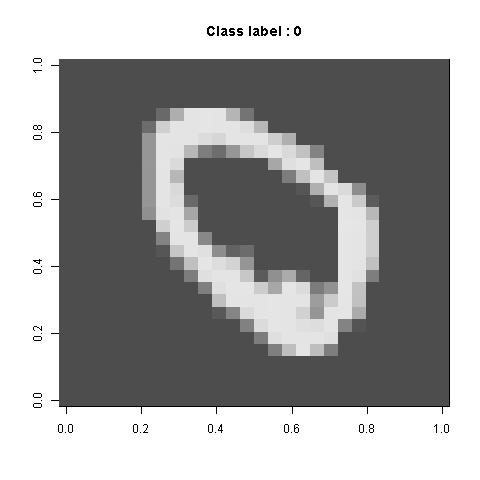
\includegraphics{0.jpg} \\
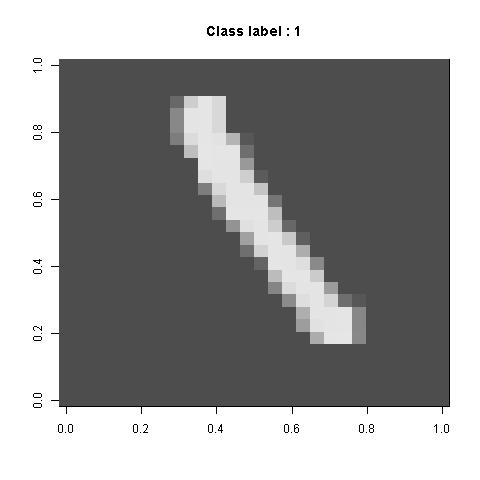
\includegraphics{1.jpg} \\
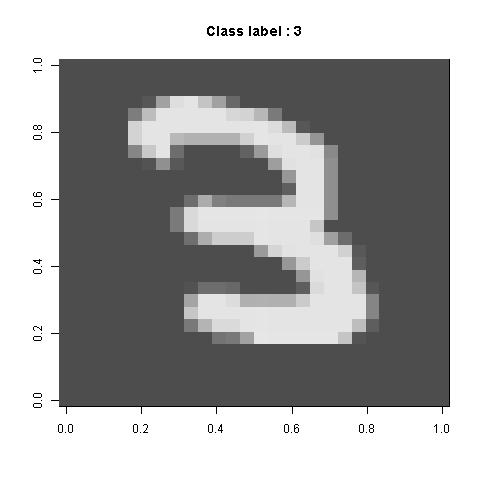
\includegraphics{3.jpg} \\
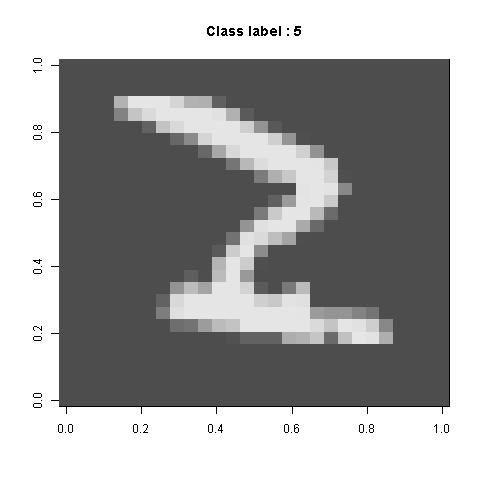
\includegraphics{5.jpg} \\

\setcounter{secnumdepth}{1}

\section{Theory}

\textbf{a} Write down the formula for computing the gradient of the loss function used in Logistic Regression. Specify what each variable represents in the equation.\\

The formula for the gradient descent is:
\[
\theta_j \leftarrow \theta_j - \alpha \sum_{i=1}^{n} \frac{1}{1 + \exp(-y^{(i)} <\theta, x^{(i)}> )}
\]
where $x^{(i)}$ is the data point represented in a vector of features, $y^{(i)}$ is the class label, and $\theta$ is the parameter vector. The goal is to reach the $\theta$ that maximizes our likelihood function (given the data we use to train the model).\\

\textbf{b} Write pseudocode for training a model using Logistic Regression.\\

\SetEndCharOfAlgoLine{}

\begin{algorithm}[H]
 \KwData{Training data}
 convergence threshold: $\eta$\;
 step size: $\alpha$\;
 \For{$j\leftarrow 0$ \KwTo $d$}{
  initialize $\theta_j$\;
  initialize $\Delta\theta_j$\;
 }
 
  \For{$i\leftarrow 1$ \KwTo $n$}{
  $x_0^{(i)} = 1$\;
 }
 \While{$\cup_{j\in\{0,1,...,d\}}|\delta\theta_j/\theta_j|>\eta$}{
    \For{$i\leftarrow 1$ \KwTo $n$}{
      $z^{(i)} = \sum_{j=0}^{d} \theta_j x_j^{(i)} $\;
      }
    \For{$j\leftarrow 0$ \KwTo $d$}{
      $\Delta = 0$\;
        \For{$i\leftarrow 1$ \KwTo $n$}{
            $\Delta \leftarrow \Delta + \frac{y^{(i)} x_j^{(i)}}{1 + \exp(-y^{(i)} z^{(i)} )}$\;
          }
      }
      $\theta_j \leftarrow $\theta_j - \alpha\Delta$\;
      $\delta\theta_j = \alpha\Delta$\;
 }
  \Return $\{\theta_0,...,\theta_d\}$\;
\end{algorithm}\DecMargin{1em}

\textbf{c} Calculate the number of operations per gradient descent iteration.\\
Each gradient descent update iteration requires $2n(d + 1)$\\

\section{Implementation}
\begin{Schunk}
\begin{Sinput}
> # Gredient Descent
> gradient_descent <- function(X, Y, XY, theta){
+     z <- as.matrix(X) %*% theta
+     yz_exp <- 1 / (1 + exp(-Y * z))
+     # Precalculate that instead for performance
+     #tmp <- apply(X,2,function(x) X * Y)
+     delta_theta <- t(XY) %*% yz_exp
+     return(delta_theta)
+ }
> # Logistic Regression
> # threshold should be higher than 100 but I used 100 by default to speed up the calculations need for the report
> logistic_regression <- function(X, Y, deviation, alpha, eta, seed = 100, threshold = 100) {
+   # initializations
+   set.seed(seed)
+   X$intercept <- 1
+   theta <- rnorm(ncol(X), sd = deviation)
+   delta_theta <- rep(10000, ncol(X))
+   numIterations <- 1
+   
+   #XY <- apply(X,2,function(x) X * Y)
+   XY <- sweep(X, 1,Y, "*")
+   while (any(abs(alpha * delta_theta/(theta + 0.0001)) > eta) & numIterations < threshold){
+     delta_theta <- gradient_descent(X,Y, XY,theta)
+     theta <- theta - alpha * delta_theta
+     numIterations <- numIterations + 1
+   }
+   return(theta)
+ }
\end{Sinput}
\end{Schunk}

\section{Training}
\textbf{a} Train 2 models, one on the train_0_1 set and another on train_3_5, and report the\\
training and test accuracies.
\begin{Schunk}
\begin{Sinput}
> # Calculate the predictions
> predict <- function(thetasFromTraining, classLabel){
+   classLabel$intercept <- 1
+   -sign(as.matrix(classLabel) %*% thetasFromTraining)
+ }
> # Calculate the accuracy
> accuracy <- function(model_function, X, Y, deviation, alpha = 0.001, eta = 0.000001, seed = 100, threshold = 100){
+   model_output <- model_function(X, Y, deviation, alpha, eta, seed, threshold)
+   a <- predict(model_output, X)
+   tmp <- mean(Y == a)
+   return(tmp)
+ }
> theta <- rnorm(ncol(train_0_1), sd = 0.5)
> accuracy(logistic_regression, train_0_1, true_label_train_0_1, deviation = 0.5)
\end{Sinput}
\begin{Soutput}
[1] 0.5323332
\end{Soutput}
\begin{Sinput}
> accuracy(logistic_regression, train_3_5, true_label_train_3_5, deviation = 0.5)
\end{Sinput}
\begin{Soutput}
[1] 0
\end{Soutput}
\end{Schunk}

\textbf{b} Repeat 3a 10 times, i.e. you should obtain 10 train and test accuracies for each set.
Calculate the average train and test accuracies over the 10 runs, and report them.

\begin{Schunk}
\begin{Sinput}
> train_0_1_accuracies <- numeric()
> for(i in 1:10){ 
+   train_0_1_accuracies <- append(train_0_1_accuracies, accuracy(logistic_regression, train_0_1, true_label_train_0_1, deviation = 0.5 ))
+ }